\documentclass[a4paper,10pt]{article}
\usepackage{amsmath,amssymb,graphicx,float,subfig}

%defines
\def\bY{{\bf Y}}
\def\bA{{\bf A}}
\def\bB{{\bf B}}
\def\bX{{\bf X}}
\def\bH{{\bf H}}
\def\bE{{\bf E}}
\def\bI{{\bf I}}
\def\bG{{\bf G}}
\def\bV{{\bf V}}
\def\bQ{{\bf Q}}
\def\btQ{{\bf \tilde Q}}
\def\bC{{\bf C}}
\def\btA{{\bf \tilde A}}
\def\b1{{\bf 1}}
\def\bx{{\bf x}}
\def\bb{{\bf b}}
\def\be{{\bf e}}
\def\bw{{\bf w}}
\def\by{{\bf y}}
\def\bz{{\bf z}}
\def\btx{{\bf{\tilde x}}}
\def\blambda{{\boldsymbol \lambda}}
\def\bgamma{{\boldsymbol \gamma}}
\def\btheta{{\boldsymbol \theta}}
\def\bbeta{{\boldsymbol \beta}}
\def\bnu{{\boldsymbol \nu}}
\def\bmu{{\boldsymbol \mu}}
\def\sigmaeps{{\sigma_{\epsilon}}}
\def\bxmode{{\hat \bx^{(0)}}}
\def\txmode{{\tilde \bx_{\mathrm{mode}}}}
\def\txsample{{\tilde \bx_{\mathrm{sample}}}}

%opening
\title{Home Assignment - 3}
\author{Santhosh Nadig, Zhanzhang Cai}

\begin{document}

\maketitle

\section{Introduction}
In this project, we consider the problem of reconstructing an image which is corrupted by random (uniform) noise using a Bayesian hierarchical model framework. The corrupted image is observed with a small additive white Gaussian noise. We use a Gaussian Markov Random Field (GMRF) SAR-model as prior for the image. In addition, a set of latent indicators indicate whether the pixel is corrupted. A Gibbs sampler is implemented to sample the parameters of the model from their conditional posteriors which enables us to re-construct the image (posterior image).

\section{Data and Model}
The input is a 215-by-126 pixel RGB image. The pixels in the input image are assumed to be corrupted independently by uniform random noise with probability ($1-p_c$) and a noisy version of this corrupted image (additive white Gaussian noise with variance $\sigmaeps^2$) is observed. The corrupted pixel locations and the variance of the observation noise are unknown and need to be estimated.

The proposed Bayesian hierarchical model is as follows: A latent field $\bx$ which is a Matern GMRF (SAR-model) is used as prior for the image. Thus, we may express $\bx$ as
\begin{equation}
 \bx \in N(\bmu, \bQ^{-1})
 \label{eq:latentfield}
\end{equation}
where $\bQ$ is a SAR precision matrix which is parametrized as 
\begin{equation*}
 \bQ = \tau \bQ_0
\end{equation*}
where $\bQ_0 = (\kappa^2 \bI - \bG)^T (\kappa^2 \bI - \bG)$ with $\kappa$ begin fixed apriori [lecture 6].

A latent indicator field $\bz$ indicates whether or not a pixel is corrupted. The prior distribution for $\bz(s)$ is $p(\bz(s)) = 0$ with probability $p_c$ and $p(\bz(s) = 1)$ with probability $(1-p_c)$. Therefore, given the latent image and indicators, the observation for each pixel can be written as
\begin{equation}
 y(s)|\bx,\bz \in \begin{cases}
                   N(x(s), \sigmaeps^2),\quad \mathrm{if }~ z(s) = 0,\\
                   U(0,1), \quad \mathrm{if }~ z(s) = 1.
                  \end{cases}
\end{equation}

To proceed with parameter estimation and reconstruction, the first step is to fix the parameter $\kappa$. This is done by obtaining a binned covariance function using the residuals $\by - \bE(\by)$. 

TBD:Figure

The estimation of the posterior image (reconstruction) is explained in the next section.

\section{Theory}
Let $\bA$ represent the observation matrix (with all the pixels) and let $\btA = \begin{bmatrix} \bA & \mathbf{1} \end{bmatrix}$. Furthermore, denote $\btA(z) = \begin{bmatrix} \bA(\bz) & \bf{1}\end{bmatrix}$, the observation matrix that is constructed with the ``uncorrupted'' pixels (i.e., where $\bz(s) = 1$) which in turns depends upon the latent field $\bz$. We denote the set of parameters  $\btheta = \{ \sigmaeps^2, \kappa, \tau, p_c\}$ represent the set of parameters. The posterior of the parameters and the latent fields can be written as
\begin{align}
 p(\bx, \bz, \btheta | \by) &\propto p(\by | \bx, \bz, \btheta) \cdot p(\bx|\btheta) \cdot p(\bz|\btheta) \nonumber \\
 &= p(\by | \bx, \bz, \sigmaeps^2) \cdot p(\bx|\kappa, \tau) \cdot p(\bz|p_c)
\end{align}
An expression for each of the conditional posteriors is elaborated in the subsequent sections.
\subsection{Conditional Posteriors}
\subsubsection{$p(\bx|\bz,\btheta,\by)$}
Assuming a constant but unknown mean value $\beta$ for the latent field $\bx$, we have
\begin{equation}
 \underbrace{\begin{bmatrix}
              \bx \\
              \beta
             \end{bmatrix}
}_{\btx} = N\left( \bf{0}, \underbrace{\begin{bmatrix}
                                  \bQ & 0 \\
                                  0 & \bQ_{\beta}
                                 \end{bmatrix}^{-1}}_{\btQ^{-1}} \right).
\end{equation}
where $\bQ_{\beta} =  \mathbb{I}\cdot 10^{-6}$. The observation likelihood can therefore be expressed as
\begin{equation}
 \by|\btx, \bz \in N(\btA\btx, \bQ_{\epsilon}^{-1}).
\end{equation}
The posterior for $\btx$ given $\by$ is given by [slide 16, lecture 7]
\begin{equation}
 \btx|\by, \btheta = N(\mu_{x|y} (\btheta), \bQ_{x|y}(\btheta)^{-1}) 
\end{equation}
where
\begin{align}
 \mu_{x|y} (\btheta) &=  \bQ_{x|y}(\btheta)^{-1} \btA^T \bQ_{\epsilon} (\btheta) \by \nonumber \\
 \bQ_{x|y}(\btheta) &= \btQ(\btheta) + \btA^T \bQ_{\epsilon}\btA.
\end{align}

\subsubsection{$p(\bz|\bx,\btheta,\by)$}
The posterior $p(\bz|\bx,\btheta,\by)$ is a Bayesian classification problem. Given the parameter $p_c$, the probability of pixel having class 0 is given by
\begin{align}
 p(z_i = 0| y_i, x_i, \btheta) &= \frac{p(y_i|z_i = 0, x_i, \btheta) p(z_i = 0)}{\sum_{k = 0}^1 p(y_i|z_i = k, x_i, \btheta) p(z_i = k)} \nonumber \\
 &= \frac{p_N(y_i|x_i,\btheta) p_c}{p_N(y_i|x_i,\btheta) p_c + (1-p_c)}
 \label{eq:bhmclass}
\end{align}
where
\begin{equation}
 p_N(y_i|x_i,\btheta) = \frac{1}{(2\pi \sigmaeps^2)^{1/2}} \exp\left( - \frac{(y_i - \mu_i)^2}{2\sigmaeps^2} \right)
\end{equation}
where $\mu_i = x_i + \beta$.

\subsubsection{$p(\sigmaeps^2|\bx,\bz,\by)$}
The posterior $p(\sigmaeps^2|\bx,\bz,\by)$ can be expressed as
\begin{align}
 p(\sigmaeps^2|\bx,\bz,\by) &\propto p(\by|\sigmaeps^2, \bmu) \nonumber \\
 &= \prod_{i=1}^n \frac{1}{(2\pi \sigmaeps^2)^{1/2}} \exp \left( -\frac{(y_i - \mu_i)^2}{2\sigmaeps^2} \right) \nonumber \\
 &\propto \frac{1}{(\sigmaeps^2)^{n/2}} \exp \left(- \sum_{i=1}^n \frac{(y_i - \mu_i)^2}{2\sigmaeps^2} \right)
\end{align}
where $n$ represents the number of ``good'' pixels (i.e., for which $\bz(s) = 0$). Comparing the above expression to a standard inverse-Gamma distribution, we obtain the parameters
\begin{align}
 \alpha &= \frac{n}{2}-1 \nonumber \\
 \beta &= \frac{\sum_{i=1}^n(y_i - \mu_i)^2}{2}
\end{align}

\subsubsection{$p(\tau|\bx,\bz,\by)$}
The latent-field $\bx$ is assumed to be drawn according to equation (\ref{eq:latentfield}) implying that the conditional posterior of $\tau$ only depends on $\bx$ and can therefore be written as
\begin{align}
 p(\tau|\bx,\bz,\by) &\propto p(\bx|\tau) \nonumber \\
 &\propto |\bQ(\kappa,\tau)|^{1/2} \exp \left( -\frac{1}{2} \bx^T \bQ(\kappa,\tau) \bx \right).
\end{align}
where $\bQ(\kappa,\tau) = \tau \bQ_0(\kappa)$. Thus
\begin{equation}
 p(\tau|\bx,\bz,\by) \propto \tau^{N/2} |\bQ_0(\kappa)|^{1/2}  \exp \left( - \tau \frac{\bx^T \bQ_0(\kappa) \bx}{2} \right)
\end{equation}
Comparing the above with a standard Gamma-distribution, one obtains the parameters as
\begin{align}
 \alpha &= \frac{N}{2} + 1 \nonumber  \\
 \beta &= \frac{\bx^T \bQ_0(\kappa) \bx}{2}
\end{align}

\subsubsection{$p(p_c | \bx, \bz, \by)$}
The posterior for $p_c$ can be expressed as
\begin{equation}
 p(p_c | \bx, \bz, \by) \propto p(\bz | p_c)
\end{equation}
Supposing there are $k$ pixels that belong to class 0, we may write
\begin{equation}
 p(\bz | p_c) \propto p_c^k (1 - p_c)^{N-k}
\end{equation}
The above expression resembles the density function of a Beta-distribution. A general Beta distribution with parameters $\alpha$ and $\beta$ and support $x \in [0,1]$ is given by
\begin{equation}
 p_{\mathrm{Beta}}(x|\alpha,\beta) = \frac{\Gamma(\alpha+\beta)}{\Gamma(\alpha) \Gamma(\beta)} x^{\alpha-1} (1-x)^{\beta-1}
\end{equation}
Comparing the two equations above, we have the parameters
\begin{equation}
 \alpha = k + 1, \quad \beta = N-k+1.
\end{equation}

\subsubsection{Gibbs Sampler}
The Gibbs Sampler algorithm sequentially samples from the conditional posteriors described above. The posterior image is reconstructed after the final iteration of the Gibbs sampler as
\begin{equation}
 \hat \by = \bA \bx + \beta \mathbf{1}.
\end{equation}

\section{Results}
For the first experiment, we choose to add 10\% corrupted pixels and $\sigmaeps^2 = 1e-4$. The reconstructed image and estimated parameters are plotted in figures (\ref{fig:img10}) and (\ref{fig:param10}) respectively. In figure (\ref{fig:img10})(c) (bottom-left), the reconstructed image has enhanced shadows and reduced sharpness due to the structure of the $\bQ$ matrix.

For the second experiment, the observation noise level was retained as before, but the corrupted pixels were increased to 25\%. The results are shown in figures (\ref{fig:img25}) and (\ref{fig:param25}) respectively.

We measured the sum of squared errors between (a) original image and observed image (with noise and corrupted pixels), and (b) original image and the reconstructed image for 10\%, 25\% and 50\% corrupted pixels and same measurment noise level as before. The results are plotted in figure (\ref{fig:sse}). Although, it appears that the recovery at 50\% corrupted pixels is pretty good, the final image is not visually acceptable.
\begin{figure}[H]
 \centering
 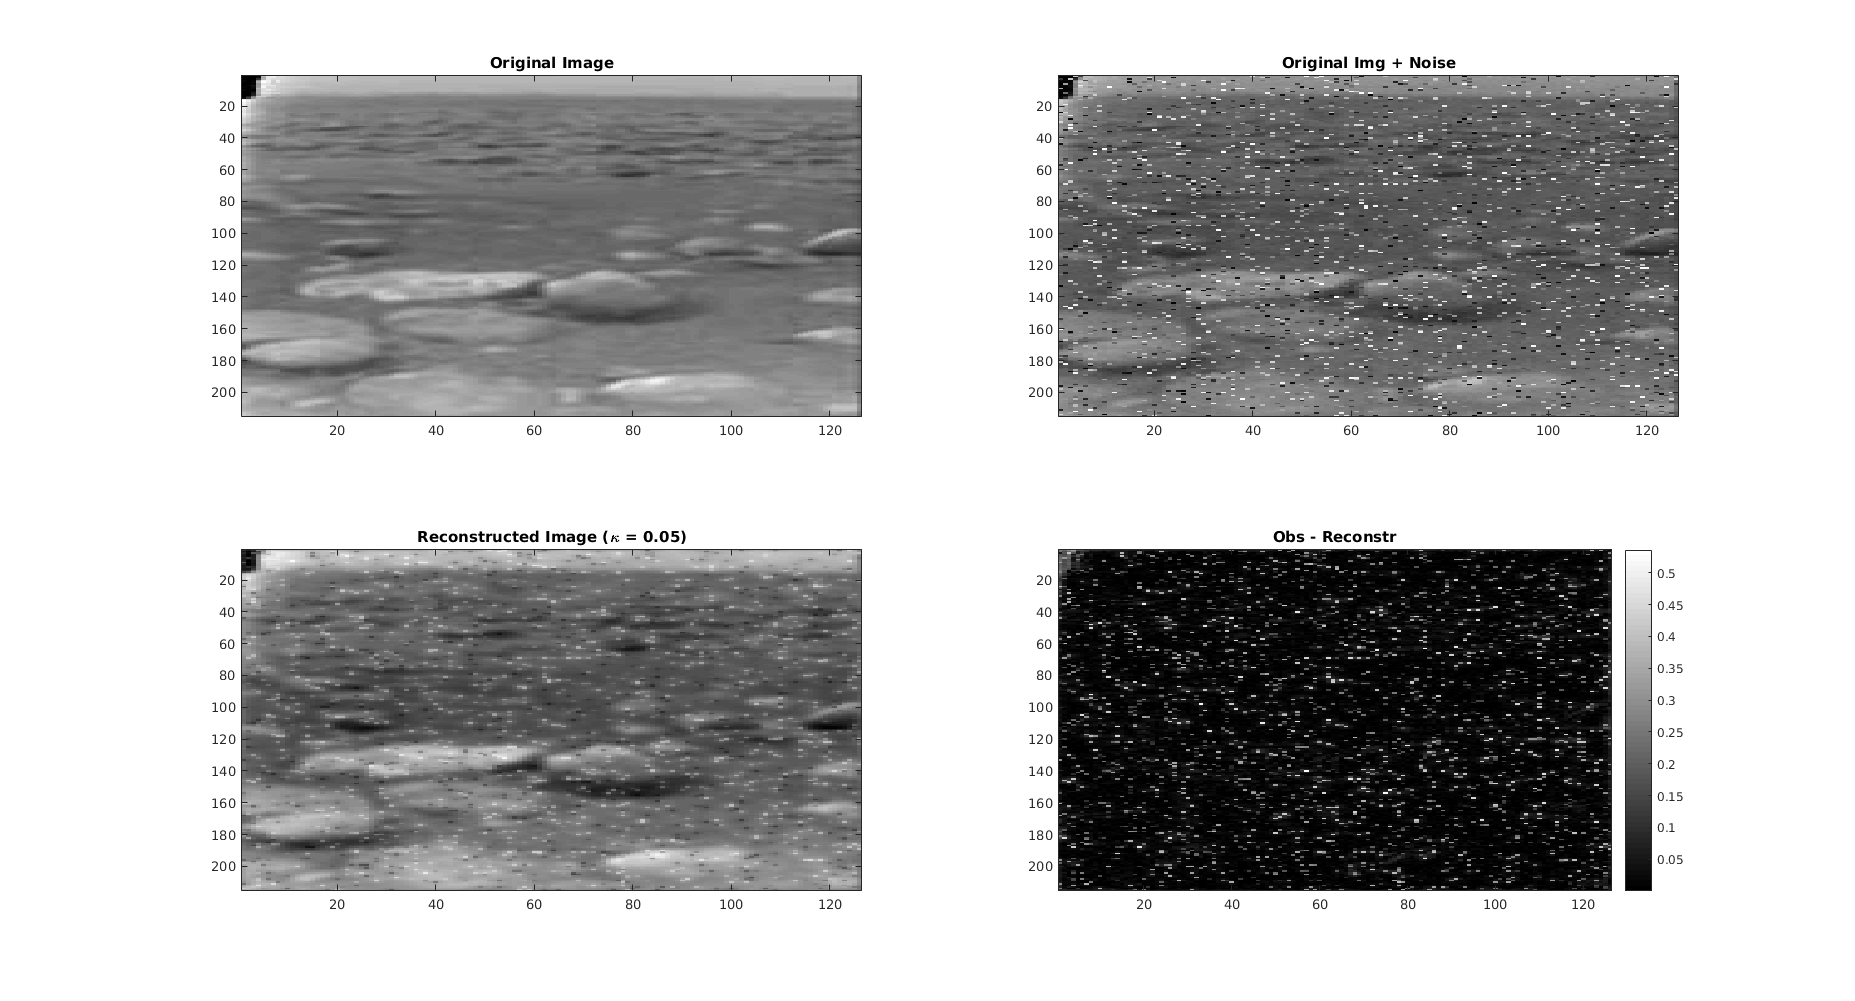
\includegraphics[width=8cm, height=8cm]{image.png}
 \caption{Reconstruction of image with 10\% corrupted pixels and observation noise of $\sigmaeps^2 = 1e-4$.}
 \label{fig:img10}
\end{figure}
\begin{figure}[H]
 \centering
 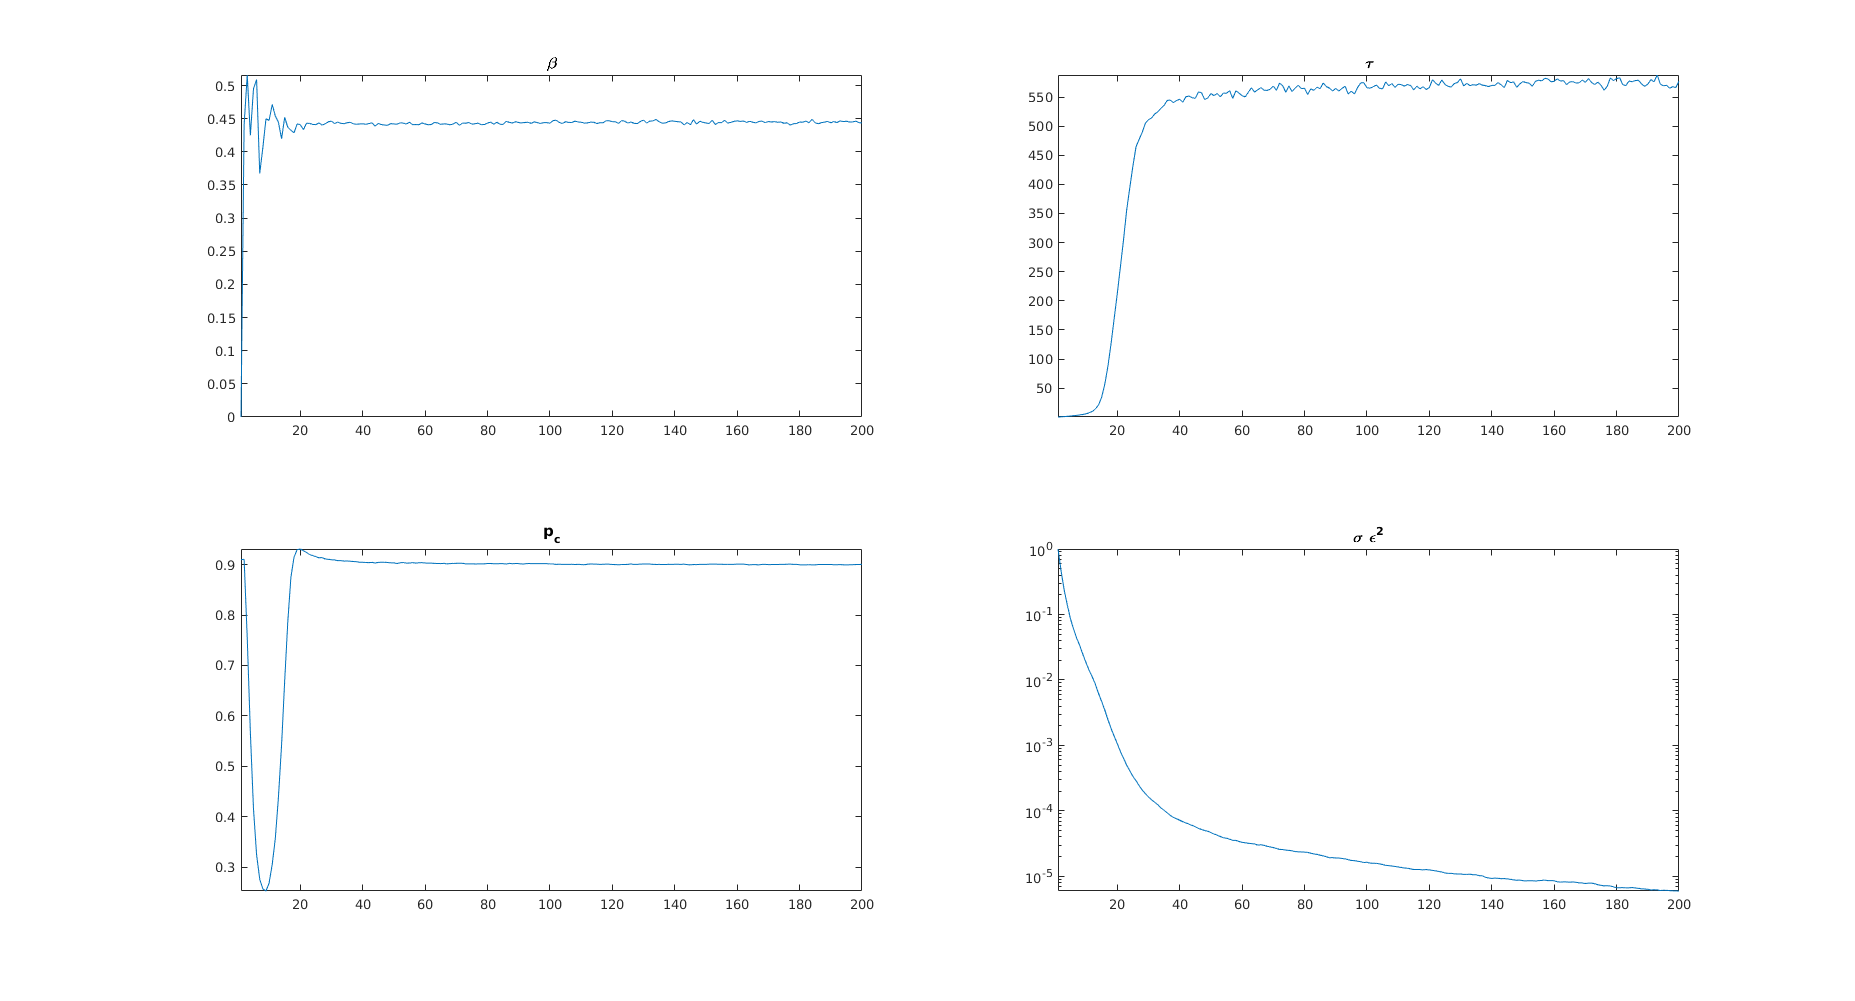
\includegraphics[width=8cm, height=8cm]{params.png}
 \caption{Parameter value vs. iterations of the Gibbs sampler.}
 \label{fig:param10}
\end{figure}
\begin{figure}[H]
 \centering
 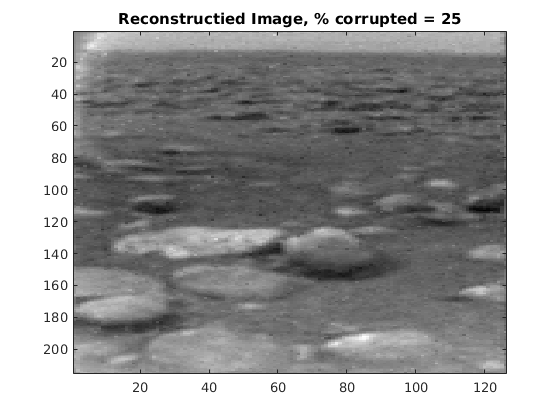
\includegraphics[width=8cm, height=8cm]{image_n25.png}
 \caption{Reconstruction of image with 25\% corrupted pixels and observation noise of $\sigmaeps^2 = 1e-4$.}
 \label{fig:img25}
\end{figure}
\begin{figure}[H]
 \centering
 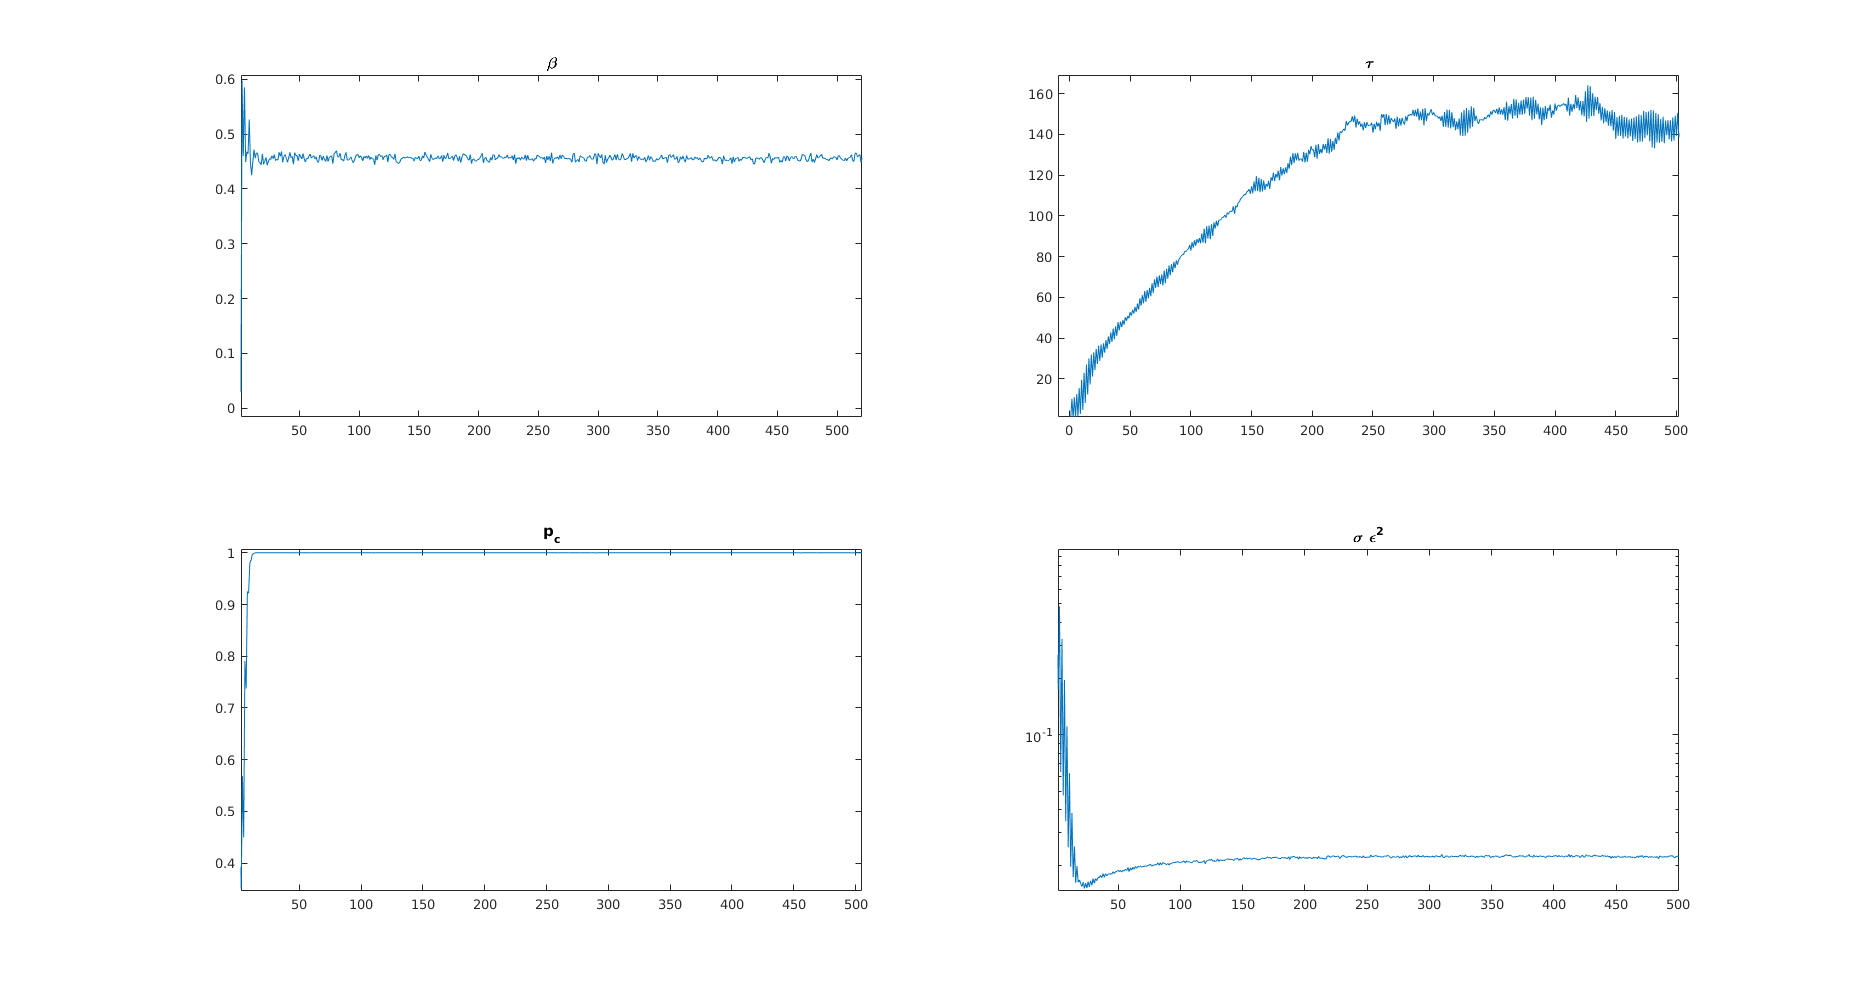
\includegraphics[width=8cm, height=8cm]{params_n25.png}
 \caption{Parameter value vs. iterations of the Gibbs sampler.}
 \label{fig:param25}
\end{figure}

\begin{figure}[H]
 \centering
 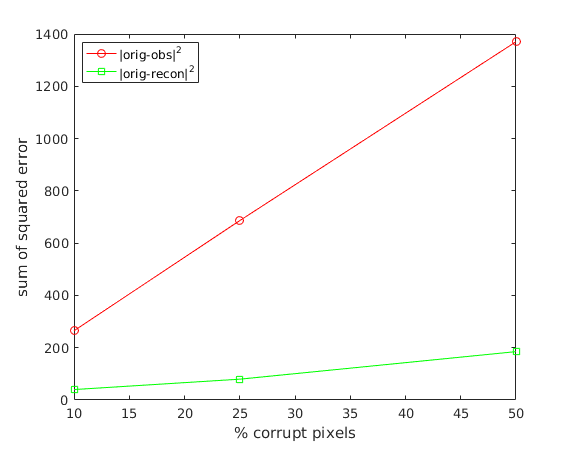
\includegraphics[width=8cm, height=8cm]{sse.png}
 \caption{Plot of sum of squared error. The red curve is the sum of squared difference between original and observed images. The green curve is the sum of squared difference between the original and reconstructed images.}
 \label{fig:sse}
\end{figure}
\end{document}
